\documentclass[oneside,openany,headings=optiontotoc,11pt,numbers=noenddot]{scrreprt}

\usepackage[a4paper]{geometry}
\usepackage[utf8]{inputenc}
\usepackage[T1]{fontenc}
\usepackage{lmodern}
\usepackage[ngerman]{babel}
\usepackage{ngerman}

\usepackage[onehalfspacing]{setspace}

\usepackage{fancyhdr}
\usepackage{fancybox}

\usepackage{rotating}
\usepackage{varwidth}

%Struktogramme
\usepackage[german,curves]{struktex}

\usepackage{pdflscape}
\usepackage{changepage}
\usepackage{graphicx}
\usepackage[bottom]{footmisc}
\usepackage{transparent}
\usepackage{graphbox}
\graphicspath{
	{Pics/PDFs/}
	{Pics/JPGs/}
	{Pics/PNGs/}
}
\usepackage{caption}
\usepackage{wrapfig}
\usepackage{marginnote}
\usepackage{tabularx}
\usepackage{dashrule}
\usepackage{soulutf8}
\usepackage{hhline}
%arydshln suppresses vertical lines in table
%\usepackage{arydshln}
\usepackage{multirow}
\usepackage{enumerate}
\usepackage[hidelinks]{hyperref}
\usepackage{listings}

\usepackage[table]{xcolor}
\usepackage{array}
\usepackage{enumitem,amssymb,amsmath}
\usepackage{interval}
\usepackage{cancel}
\usepackage{stmaryrd}
\usepackage{wasysym}
\usepackage{polynom}
\usepackage{diagbox}
\usepackage{dashrule}
\usepackage{framed}
\usepackage{mdframed}
\usepackage{karnaugh-map}
\usepackage{pdfpages}

\usepackage{blindtext}

\usepackage{eso-pic}

\usepackage{amssymb}
\usepackage{eurosym}

\usepackage[pages=some]{background}
\pagestyle{headings}
\renewcommand{\headrulewidth}{0.2pt}
\renewcommand{\footrulewidth}{0.2pt}
\newcommand*{\underdownarrow}[2]{\ensuremath{\underset{\overset{\Big\downarrow}{#2}}{#1}}}
\setlength{\fboxsep}{5pt}
\newcommand{\explainBelow}[3]{\underbrace{#1}_{\parbox{\widthof{#3}}{\footnotesize\raggedright #2}}}
\newcommand{\explainAbove}[3]{\overbrace{#1}^{\parbox{\widthof{#3}}{\footnotesize\raggedright #2}}}
\newcommand\footnoteref[1]{\protected@xdef\@thefnmark{\ref{#1}}\@footnotemark}


% Codestyle defined
\definecolor{codegreen}{rgb}{0,0.6,0}
\definecolor{codegray}{rgb}{0.5,0.5,0.5}
\definecolor{codepurple}{rgb}{0.58,0,0.82}
\definecolor{backcolour}{rgb}{0.95,0.95,0.92}
\definecolor{deepgreen}{rgb}{0,0.5,0}
\definecolor{darkblue}{rgb}{0,0,0.65}
\definecolor{mauve}{rgb}{0.40, 0.19,0.28}
\colorlet{exceptioncolour}{yellow!50!red}
\colorlet{commandcolour}{blue!60!black}
\colorlet{numpycolour}{blue!60!green}
\colorlet{specmethodcolour}{violet}

%Neue Spaltendefinition
\newcolumntype{L}[1]{>{\raggedright\let\newline\\\arraybackslash\hspace{0pt}}m{#1}}
\newcolumntype{M}{>{\centering\arraybackslash}X}
\newcommand{\cmnt}[1]{\ignorespaces}
%Textausrichtung ändern
\newcommand\tabrotate[1]{\rotatebox{90}{\raggedright#1\hspace{\tabcolsep}}}

%Intervall-Konfig
\intervalconfig {
	soft open fences
}

%Bash
\lstdefinestyle{BashInputStyle}{
	language=bash,
	basicstyle=\small\sffamily,
	backgroundcolor=\color{backcolour},
	columns=fullflexible,
	backgroundcolor=\color{backcolour},
	breaklines=true,
}
%Java
\lstdefinestyle{JavaInputStyle}{
	language=Java,
	backgroundcolor=\color{backcolour},
	aboveskip=1mm,
	belowskip=1mm,
	showstringspaces=false,
	columns=flexible,
	basicstyle={\footnotesize\ttfamily},
	numberstyle={\tiny},
	numbers=none,
	keywordstyle=\color{purple},,
	commentstyle=\color{deepgreen},
	stringstyle=\color{blue},
	emph={out},
	emphstyle=\color{darkblue},
	emph={[2]rand},
	emphstyle=[2]\color{specmethodcolour},
	breaklines=true,
	breakatwhitespace=true,
	tabsize=2,
}
%Python
\lstdefinestyle{PythonInputStyle}{
	language=Python,
	alsoletter={1234567890},
	aboveskip=1ex,
	basicstyle=\footnotesize,
	breaklines=true,
	breakatwhitespace= true,
	backgroundcolor=\color{backcolour},
	commentstyle=\color{red},
	otherkeywords={\ , \}, \{, \&,\|},
	emph={and,break,class,continue,def,yield,del,elif,else,%
		except,exec,finally,for,from,global,if,import,in,%
		lambda,not,or,pass,print,raise,return,try,while,assert},
	emphstyle=\color{exceptioncolour},
	emph={[2]True,False,None,min},
	emphstyle=[2]\color{specmethodcolour},
	emph={[3]object,type,isinstance,copy,deepcopy,zip,enumerate,reversed,list,len,dict,tuple,xrange,append,execfile,real,imag,reduce,str,repr},
	emphstyle=[3]\color{commandcolour},
	emph={[4]ode, fsolve, sqrt, exp, sin, cos, arccos, pi,  array, norm, solve, dot, arange, , isscalar, max, sum, flatten, shape, reshape, find, any, all, abs, plot, linspace, legend, quad, polyval,polyfit, hstack, concatenate,vstack,column_stack,empty,zeros,ones,rand,vander,grid,pcolor,eig,eigs,eigvals,svd,qr,tan,det,logspace,roll,mean,cumsum,cumprod,diff,vectorize,lstsq,cla,eye,xlabel,ylabel,squeeze},
	emphstyle=[4]\color{numpycolour},
	emph={[5]__init__,__add__,__mul__,__div__,__sub__,__call__,__getitem__,__setitem__,__eq__,__ne__,__nonzero__,__rmul__,__radd__,__repr__,__str__,__get__,__truediv__,__pow__,__name__,__future__,__all__},
	emphstyle=[5]\color{specmethodcolour},
	emph={[6]assert,range,yield},
	emphstyle=[6]\color{specmethodcolour}\bfseries,
	emph={[7]Exception,NameError,IndexError,SyntaxError,TypeError,ValueError,OverflowError,ZeroDivisionError,KeyboardInterrupt},
	emphstyle=[7]\color{specmethodcolour}\bfseries,
	emph={[8]taster,send,sendMail,capture,check,noMsg,go,move,switch,humTem,ventilate,buzz},
	emphstyle=[8]\color{blue},
	keywordstyle=\color{blue}\bfseries,
	rulecolor=\color{black!40},
	showstringspaces=false,
	stringstyle=\color{deepgreen}
}

\lstset{literate=%
	{Ö}{{\"O}}1
	{Ä}{{\"A}}1
	{Ü}{{\"U}}1
	{ß}{{\ss}}1
	{ü}{{\"u}}1
	{ä}{{\"a}}1
	{ö}{{\"o}}1
}

% Neue Klassenarbeits-Umgebung
\newenvironment{worksheet}[3]
% Begin-Bereich
{
	\newpage
	\sffamily
	\setcounter{page}{1}
	\ClearShipoutPicture
	\AddToShipoutPicture{
		\put(55,761){{
				\mbox{\parbox{385\unitlength}{\tiny \color{codegray}BBS I Mainz, #1 \newline #2
						\newline #3
					}
				}
			}
		}
		\put(455,761){{
				\mbox{\hspace{0.3cm}
\includegraphics[width=0.2\textwidth]{../../logo.pdf}}
			}
		}
	}
}
% End-Bereich
{
	\clearpage
	\ClearShipoutPicture
}

\geometry{left=2.50cm,right=2.50cm,top=3.00cm,bottom=1.00cm,includeheadfoot}

\begin{document}
	\begin{worksheet}{Höhere Berufsfachschule IT-Systeme}{Grundstufe - Mathematik}{Wochenplan Quadratische Funktionen}
		\noindent
		\begin{tabularx}{\textwidth}{XXl}
			Wochenplan Nr.: \rule{0.15\textwidth}{1pt} & Erledigt: & Zeitraum: \underline{29.10 - 02.11}
		\end{tabularx}
	
		\begin{framed}
			\noindent
			\textbf{Teil 1:} Legen Sie für die folgenden Funktionen eine Wertetabelle an:\\
			\par\noindent
			(a) \(f(x) = 2x^2 - 8x +6\)\\
			\par\noindent
			\begin{tabularx}{\textwidth}{X|X|X|X|X|X}
				x & \(0\) & \(1\) & \(2\) & \(3\) & \(4\)\\
				\hline
				y & \(6\) & \(0\) & \(-2\) & \(0\) & \(6\)\\
			\end{tabularx}\\
			\par\noindent
			(b) \(f(x) = -x^2 + 4\)\\
			\par\noindent
			\begin{tabularx}{\textwidth}{X|X|X|X|X|X}
				x & \(-2\) & \(-1\) & \(0\) & \(1\) & \(2\)\\
				\hline
				y & \(-8\) & \(-5\) & \(-4\) & \(-5\) & \(-8\)\\
			\end{tabularx}\\
			\par\noindent
			(c) \(f(x) = \frac{1}{4}x^2 -2x + \frac{15}{4}\)\\
			\par\noindent
			\begin{tabularx}{\textwidth}{X|X|X|X|X|X}
				x & \(-2\) & \(-1\) & \(0\) & \(1\) & \(2\)\\
				\hline
				y & \(8,75\) & \(6\) & \(3,75\) & \(2\) & \(0,75\)\\
			\end{tabularx}\\
		\end{framed}
		\begin{framed}
			\noindent
			\textbf{Teil 2:} Überführen Sie die Funktionen aus \textbf{Teil 1} in Scheitelpunktform\\
			(\(f_{SP}(x) = a\cdot(x - x_{SP}) + y_{SP}\)).\\
			\par\noindent
			Um von der \underline{allgemeinen Form} in die \textbf{Scheitelpunktform} zu gelangen, nutzen wir die quadratische Ergänzung.\\
			(a) \(f(x) = 2x^2-8x+6\)\\
			\begin{align*}
				& = 2\cdot{}(x^2-4x+3)\\
				& = 2\cdot{}(x^2 - 2\cdot{}\colorbox{green!10}{2}x & +3)\\
				& = 2\cdot{}(x^2 - 2\cdot{}\colorbox{green!10}{2}x + \underbrace{2^2 - 2^2}_{Addition\ von\ 0} & + 3)\\
				& = 2\cdot{}(\underbrace{x^2-2\cdot{}2x + \colorbox{green!10}{2}^2}_{1. binomische\ Formel} -2^2 & + 3)\\
				& = 2\cdot{}[(x-\colorbox{green!10}{2})^2 - 1]\\
				& = 2\cdot{}(x-2)^2 - 2
			\end{align*}
			\par\noindent
			(b) \(f(x) = -x^2+4\)
			\begin{align*}
				& = -1\cdot{}(x^2-4)\\
				& = -1\cdot{}(x^2 + \colorbox{red!5}{2}\cdot{}\colorbox{red!5}{0x} & - 4)\\
				& = -1\cdot{}(x^2 \mathit{2\cdot{}0x} + \underbrace{0^2 - 0^2}_{Addition\ von\ 0} & - 4)\\
				& = -1\cdot{}(\underbrace{x^2 + \mathit{2\cdot{}0x} + \colorbox{green!10}{0}^2}_{1. binomische\ Formel} - 0^2 & - 4)\\
				& = -1\cdot{}[(x+\colorbox{green!10}{0})^2 - 4]\\
				& = -(x-0)^2 +4
			\end{align*}
			\par\noindent
			(c) \(f(x) = \frac{1}{4}x^2-2x+\frac{15}{4}\)
			\begin{align*}
				& = \frac{1}{4}\cdot(x^2-8x+15)\\
				& = \frac{1}{4}\cdot{}(x^2 - 2\cdot{}\colorbox{green!10}{4}x & + 15)\\
				& = \frac{1}{4}\cdot{}(x^2 - 2\cdot{}\colorbox{green!10}{4}x + \underbrace{4^2 - 4^2}_{Addition\ von\ 0} & + 15)\\
				& = 2\cdot{}(\underbrace{x^2-2\cdot{}4x + \colorbox{green!10}{4}^2}_{1. binomische\ Formel} -4^2 & + 15)\\
				& = \frac{1}{4}\cdot{}[(x-\colorbox{green!10}{4})^2 - 1]\\
				& = \frac{1}{4}\cdot{}(x-4)^2 - \frac{1}{4}
			\end{align*}
		\end{framed}
		\begin{framed}
			\noindent
			\textbf{Teil 3:} Bestimmen Sie die Funktionswerte der folgenden Funktionen für \(x = -4\), \(x = -2\), \(x = 1\), \(x = 3\) und \(x = 5\).\\
			\par\noindent
			(a) \(f(x) = 0,5\cdot(x-2)^2 + 2\)\\
			\par\noindent
			\begin{tabularx}{\textwidth}{X|X|X|X|X|X}
				x & \(-4\) & \(-2\) & \(1\) & \(3\) & \(5\)\\
				\hline
				y & \(20\) & \(10\) & \(2,5\) & \(2,5\) & \(6,5\)\\
			\end{tabularx}\\
			\par\noindent
			(b) \(f(x) = 2\cdot(x-2)(x+4)\)\\
			\par\noindent
			\begin{tabularx}{\textwidth}{X|X|X|X|X|X}
				x & \(-4\) & \(-2\) & \(1\) & \(3\) & \(5\)\\
				\hline
				y & \(0\) & \(10\) & \(-10\) & \(14\) & \(54\)\\
			\end{tabularx}\\
			\par\noindent
			(c) \(f(x) = -x^2 + 8x -16\)\\
			\par\noindent
			\begin{tabularx}{\textwidth}{X|X|X|X|X|X}
				x & \(-4\) & \(-2\) & \(1\) & \(3\) & \(5\)\\
				\hline
				y & \(-64\) & \(-36\) & \(-9\) & \(-1\) & \(-1\)\\
			\end{tabularx}\\
			\par\noindent
			(d) \(f(x) = -2\cdot(x+4)^2 + 1\)\\
			\par\noindent
			\begin{tabularx}{\textwidth}{X|X|X|X|X|X}
				x & \(-4\) & \(-2\) & \(1\) & \(3\) & \(5\)\\
				\hline
				y & \(1\) & \(-7\) & \(-49\) & \(-97\) & \(-161\)\\
			\end{tabularx}\\
			\par\noindent
			(e) \(f(x) = x^2 + 4\)\\
			\par\noindent
			\begin{tabularx}{\textwidth}{X|X|X|X|X|X}
				x & \(-4\) & \(-2\) & \(1\) & \(3\) & \(5\)\\
				\hline
				y & \(20\) & \(8\) & \(5\) & \(13\) & \(29\)\\
			\end{tabularx}\\
			\par\noindent
			(f) \(\frac{2}{5}\cdot(x+3)(x-4)\)\\
			\par\noindent
			\begin{tabularx}{\textwidth}{X|X|X|X|X|X}
				x & \(-4\) & \(-2\) & \(1\) & \(3\) & \(5\)\\
				\hline
				y & \(3,2\) & \(-2,4\) & \(-4,8\) & \(-2,4\) & \(3,2\)\\
			\end{tabularx}\\
		\end{framed}
		\begin{framed}
			\noindent
			\textbf{Teil 4:} Geben Sie zu jeder der Funktionen aus \textbf{Teil 1} und \textbf{Teil 3} jeweils den Streckungs- bzw. Stauchungsfaktor an.\\
			Erläutern Sie jeweils, welche Aussage Sie mit ihm über den Graphen der Funktion machen können.\\
			Teil 1:\\
			\begin{tabularx}{\textwidth}{X|l|X|X}
				& \textit{a} & \shortstack{\textit{Normalparabel}\\\textit{Stauchung/Streckung}} & \textit{Aussage}\\
				\hline
				(a) \(f(x) = 2x^2 - 8x +6\) & \(a = 2\) & \(|a| > 1\), also \textbf{gestreckt} & \(a > 0\), also nach \textbf{oben} geöffnet \\
				\hline
				(b) \(f(x) = -x^2 + 4\) & \(a = -1\) & \(|a| = 1\), also \textbf{Normalparabel} & \(a < 0\), nach \textbf{unten} geöffnet \\
				\hline
				(c) \(f(x) = \frac{1}{4}x^2 -2x + \frac{15}{4}\) & \(a = \frac{1}{4}\) & \(|a| < 1\) also \textbf{gestaucht} & \(a > 0\), also nach \textbf{oben} geöffnet \\
			\end{tabularx}\\
			\newpage
			Teil 3:\\
			\begin{tabularx}{\textwidth}{X|l|X|X}
				& \textit{a} & \shortstack{\textit{Normalparabel}\\\textit{Stauchung/Streckung}} & \textit{Aussage}\\
				\hline
				(a) \(f(x) = 0,5\cdot(x-2)^2 + 2\) & \( a = 0,5\) & \(|a| < 1\), also \textbf{gestaucht} & \(a > 0\), also nach \textbf{oben} geöffnet\\
				\hline
				(b) \(f(x) = 2\cdot(x-2)(x+4)\) & \(a = 2\) & \(|a| > 1\), also \textbf{gestreckt} & \(a > 0\), also nach \textbf{oben} geöffnet\\
				\hline
				(c) \(f(x) = -x^2 + 8x -16\) & \( a = -1\) & \(|a| = 1\), also \textbf{Normalparabel} & \(a < 0\), also nach \textbf{unten} geöffnet \\
				\hline
				(d) \(f(x) = -2\cdot(x+4)^2 + 1\) & \(a = -2\) & \(|a| > 1\), also \textbf{gestreckt} & \(a < 0\), also nach \textbf{unten} geöffnet \\
				\hline
				(e) \(f(x) = x^2 + 4\) & \(a = 1\) & \(|a| = 1\), also \textbf{Normalparabel} & \(a > 0\), also nach \textbf{oben} geöffnet\\
				\hline
				(f) \(f(x) = \frac{2}{5}\cdot(x+3)(x-4)\) & \(a = \frac{2}{5}\) & \(|a| < 1\), also \textbf{gestaucht} & \(a > 0\), also nach \textbf{oben} geöffnet\\
			\end{tabularx}
		\end{framed}
		\newpage
		\begin{framed}
			\noindent
			\textbf{Teil 5:} Skizzieren Sie die Graphen der Funktionen von \textbf{Teil 1} .\\
			\begin{tabularx}{\textwidth}{XX}
				(a) 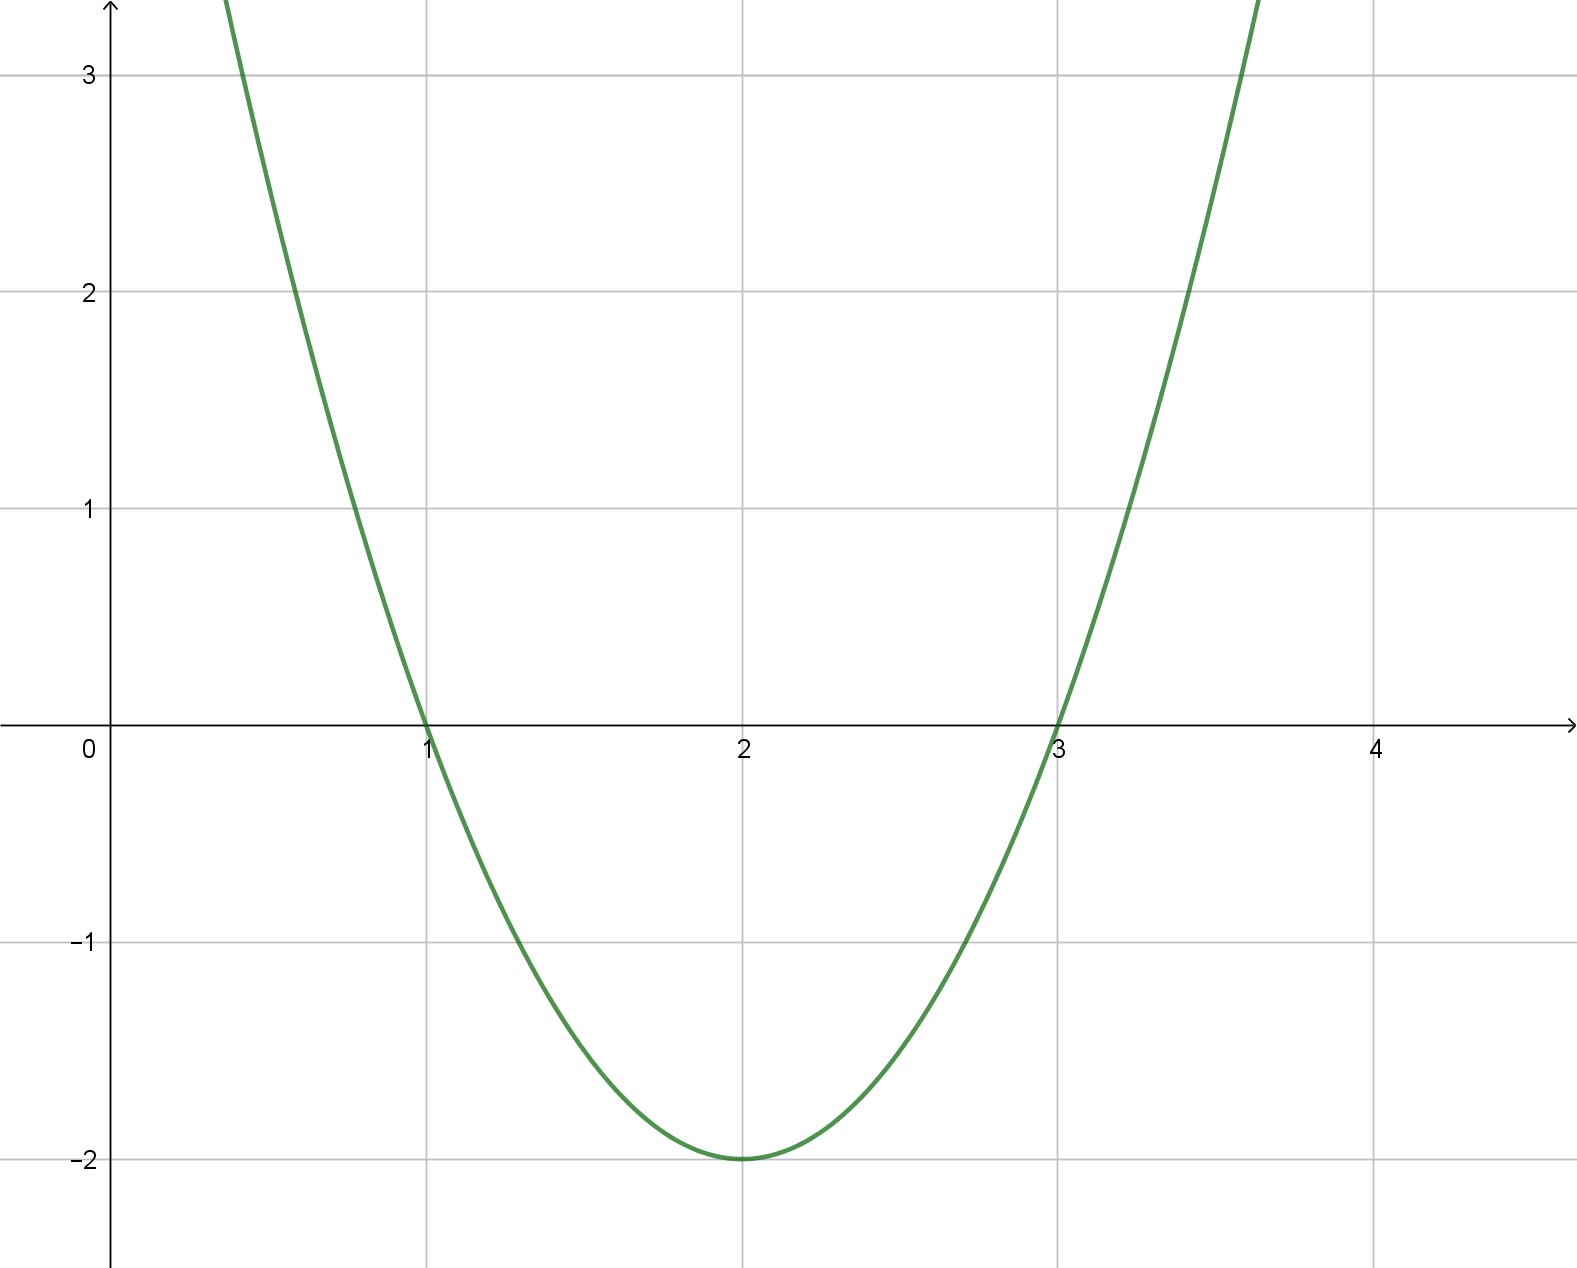
\includegraphics[width=0.4\textwidth, align=t]{../99_Bilder/WP5DiAL.jpg} & (b) 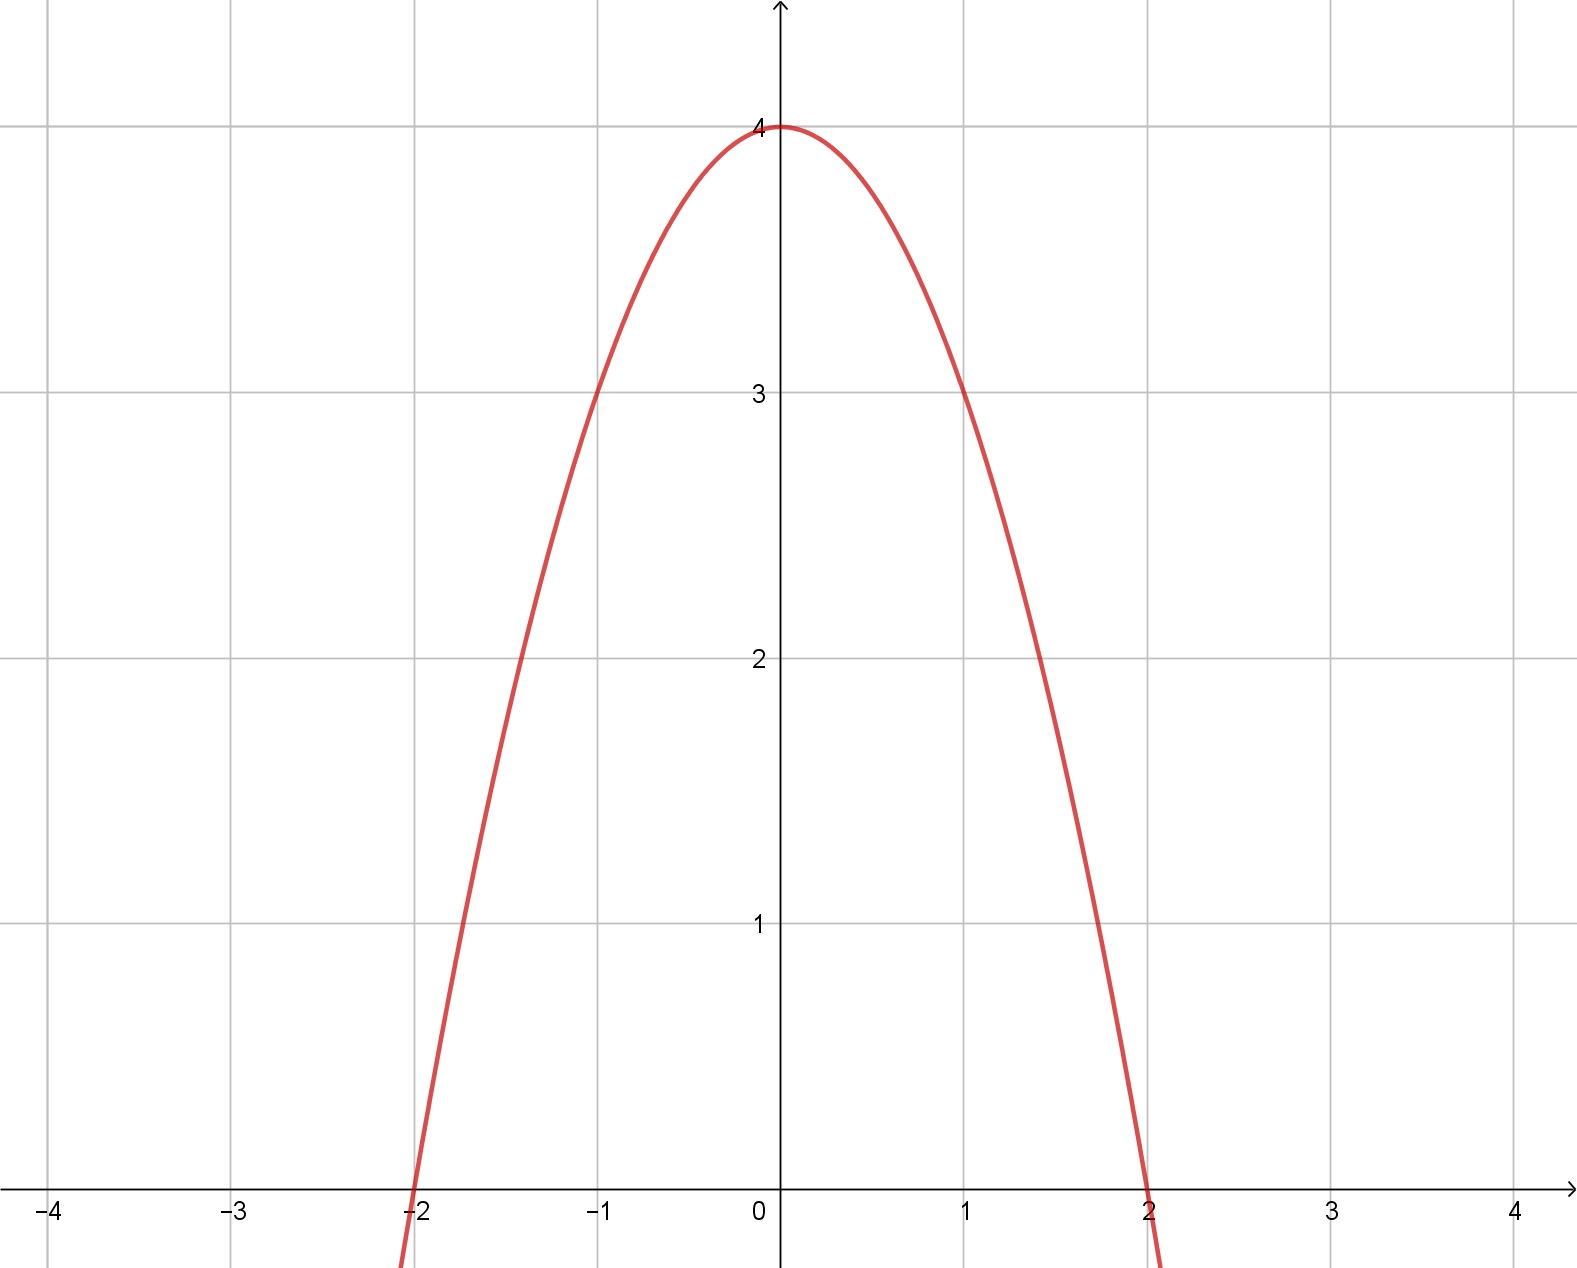
\includegraphics[width=0.4\textwidth, align=t]{../99_Bilder/WP5DiBL.jpg}\\
				\multicolumn{2}{c}{(c) 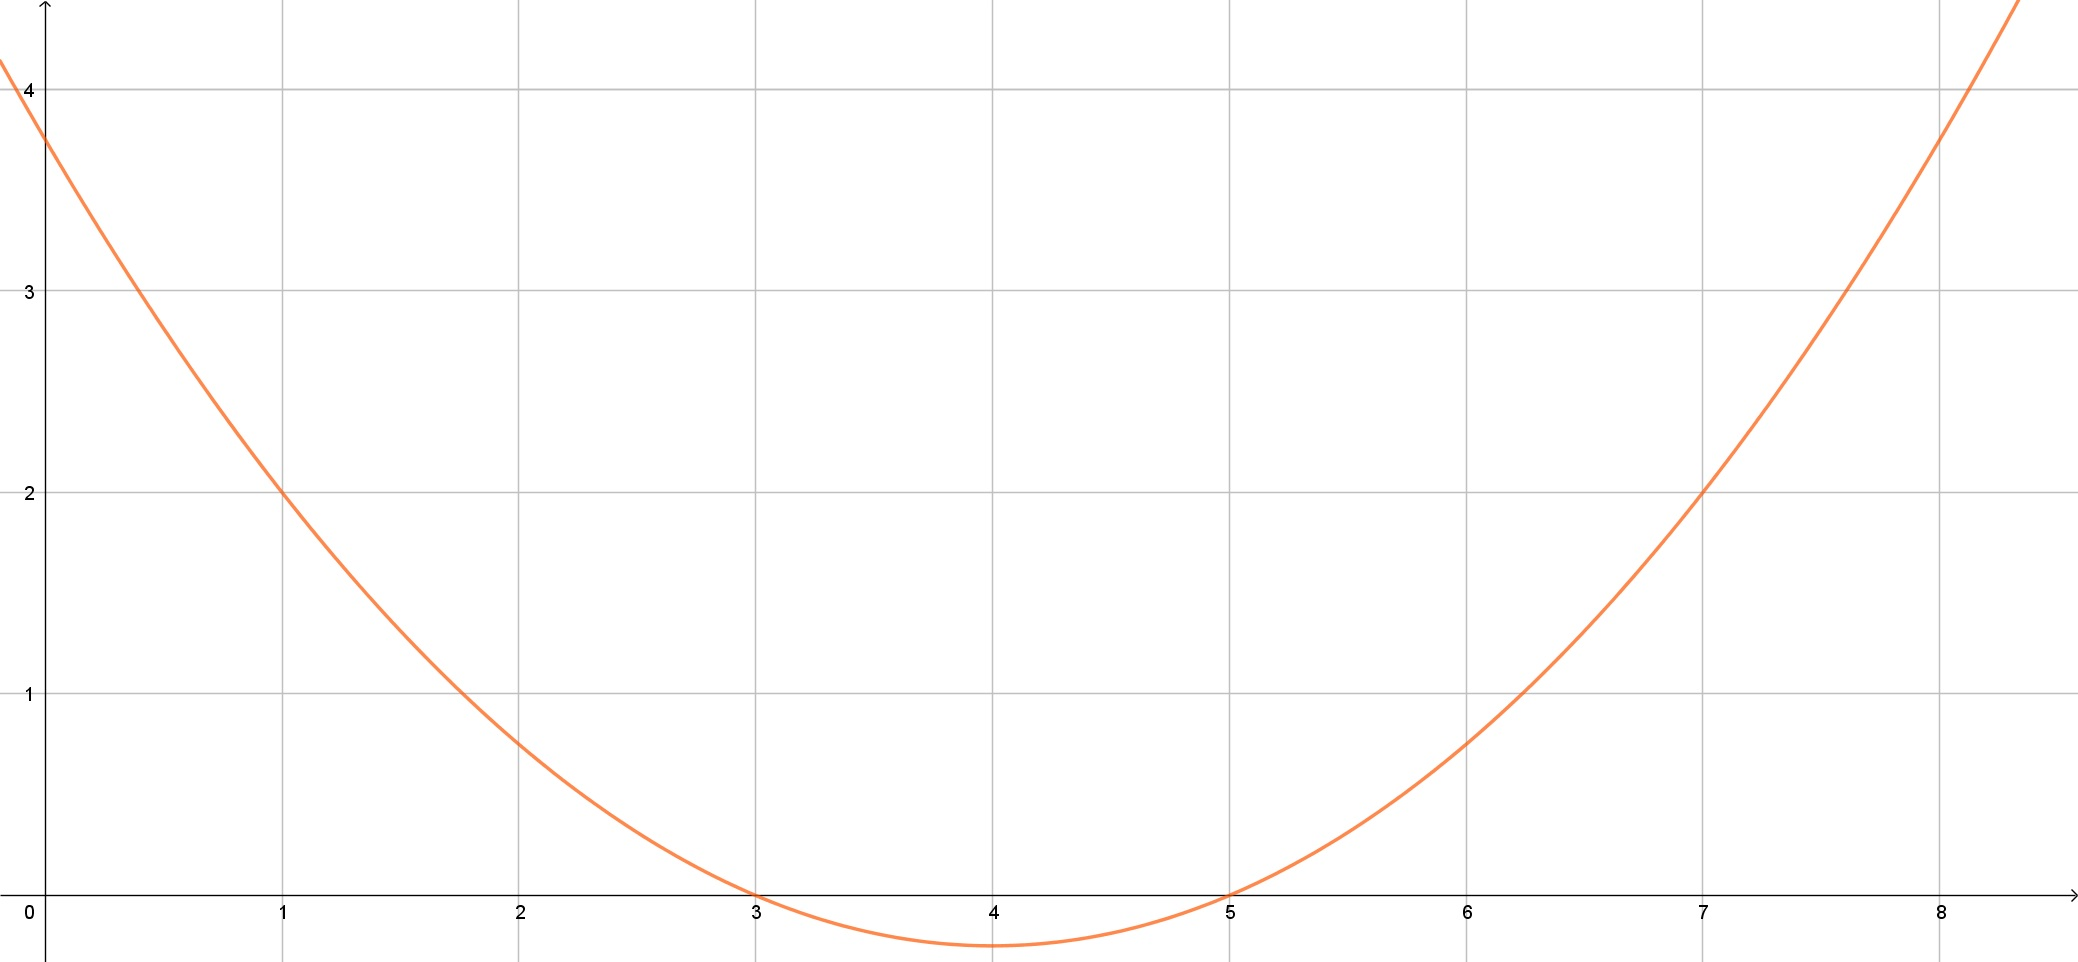
\includegraphics[width=0.8\textwidth, align=t]{../99_Bilder/WP5DiCL.jpg}}
			\end{tabularx}
		\end{framed}
	\end{worksheet}
\end{document}